\documentclass[11pt, a4paper]{article}
\usepackage[ngerman]{babel}
\usepackage[utf8]{inputenc}
\usepackage[T1]{fontenc}
\usepackage[ngerman]{babel}
\usepackage{amsmath}
\usepackage{amssymb}
\usepackage{graphicx}
\usepackage{geometry}
\usepackage{fancyhdr}
\usepackage{enumitem}
\usepackage{array}
\usepackage{eso-pic}

\usepackage{siunitx}
\DeclareSIUnit{\litre}{l}
\sisetup{angle-symbol-degree = ^\circ}
\sisetup{locale = DE, separate-uncertainty, inter-unit-product = {},
range-units = brackets, list-units = single, per-mode=symbol-or-fraction}

\makeatletter
\def\input@path{{./}{../../}}
\makeatother
\graphicspath{{./}{../../}}

\geometry{a4paper, top=2.5cm, bottom=2.5cm, left=2.5cm, right=2.5cm}

\input{defs}

\pagestyle{fancy}
\fancyhf{}
\cfoot{\thepage}

\begin{document}
\AddToShipoutPictureBG*{%
  \AtPageUpperLeft{%
    \hspace{2.0cm}%
    \raisebox{-5.cm}{%
      
\includegraphics[width=4cm]{Bilder/Allgemein/LogoFHCampus.png}%
    }%
  }%
}

\begin{center}
    {\Large \textbf{Physikalische Grundlagen}} \\[1em]
    {\large 2. Schriftliche Prüfung: Sommersemester 2026} \\[1em]
    {\large Studiengang: Clinical Engineering}
\end{center}

\vspace{1cm}

\noindent
\begin{tabular}{ll}
    \textbf{Vorname:} & \underline{\hspace{8cm}} \\[0.3cm]
    \textbf{Nachname:} & \underline{\hspace{8cm}} \\
\end{tabular}

\vspace{1cm}

\begin{itemize}[label={$\Diamond$}]
    \item Sie haben 90 min Zeit.
    \item Es sind keine Unterlagen erlaubt.
    \item Sie dürfen einen Taschenrechner verwenden.
    \item Geben Sie klare und verständliche Antworten.
    \item Schreiben Sie leserlich.
    \item Streichen Sie alle bis auf eine Lösung durch.
    \item Jeglicher Versuch unerlaubte Hilfsmittel zu verwenden oder von KommilitonInnen \\
    abzuschreiben, wird mit einer negativen Bewertung des Tests geahndet.
\end{itemize}

\vspace{1cm}

\begin{center}
    \textbf{Viel Erfolg!}
\end{center}

\vspace{2cm}

\begin{flushright}
    \renewcommand{\arraystretch}{1.23}
    \begin{tabular}{l p{2.3cm}}
        \hline
        \noalign{\vskip 0.15cm}
        \textbf{\Large{Punkte:}} & \textbf{\Large{/50}} \\
        \noalign{\vskip 0.1cm}
        \hline
        Beispiel 1: & /13 \\
        Beispiel 2: & /14 \\
        Beispiel 3: & /13 \\
        Beispiel 4: & /10
    \end{tabular}
\end{flushright}

\newpage

\section*{Beispiel 1 - Eis im Wasser}

Ein wärmeisoliertes Gefäß enthält \SI{3.0}{\litre} Wasser mit einer Anfangstemperatur von $T_{\text{W}} = \SI{40}{\degreeCelsius}$. In das Wasser werden \SI{600}{\gram} Eis mit einer Temperatur von $T_{\text{Eis}} = \SI{-10}{\degreeCelsius}$ gegeben.

Gegeben sind die spezifische Wärmekapazität von Eis $c_{\text{Eis}} = \SI{2.09}{\kilo\joule\per(\kilogram\cdot\kelvin)}$, die spezifische Wärmekapazität von Wasser $c_{\text{W}} = \SI{4.18}{\kilo\joule\per(\kilogram\cdot\kelvin)}$, die spezifische Schmelzwärme von Eis $\lambda_{\text{S}} = \SI{333.5}{\kilo\joule\per\kilogram}$ und die Dichte von Wasser $\rho_{\text{W}} = \SI{1.0}{\kilogram\per\deci\metre\cubed}$.

\subsection*{Aufgabe}
Prüfen Sie, ob das gesamte Eis schmilzt, und berechnen Sie die Endtemperatur $T_{\text{Misch}}$ des Systems.

\subsection*{Vorgehen}
\begin{enumerate}
    \item Berechnen Sie die Masse des warmen Wassers.
    \item Berechnen Sie die Wärmemenge $Q_{\text{ab,0}}$, die das warme Wasser maximal abgeben kann, wenn es bis auf \SI{0}{\degreeCelsius} abkühlt.
    \item Berechnen Sie die Wärmemenge $Q_{\text{zu,0}}$, die benötigt wird, um das gesamte Eis auf \SI{0}{\degreeCelsius} zu erwärmen und anschließend zu schmelzen.
    \item Vergleichen Sie $Q_{\text{ab,0}}$ und $Q_{\text{zu,0}}$. Entscheiden Sie, ob das gesamte Eis schmilzt, und formulieren Sie die passende Energiebilanz für den tatsächlich eintretenden Fall.
    \item Berechnen Sie die Endtemperatur $T_{\text{Misch}}$.
\end{enumerate}

\vfill
\begin{flushright}
\renewcommand{\arraystretch}{1.23}
\begin{tabular}{|c | c | c | c | c|}
\hline
\multicolumn{5}{|l|}{\textbf{\large{Punkte: \quad\quad\quad /13}}}\\
\hline
\textbf{1)} & \textbf{2)} & \textbf{3)} & \textbf{4)} & \textbf{5)} \\
\quad/2 & \quad/2 & \quad/2 & \quad/2 & \quad/5 \\
\hline
\end{tabular}
\end{flushright}

\newpage

\section*{Beispiel 2 - Auto in der Kurve}

Ein Auto mit der Masse $m = \SI{1200}{\kilogram}$ fährt auf einer ebenen Straße durch eine kreisförmige Kurve mit Radius $r = \SI{50}{\metre}$. Der Haftreibungskoeffizient zwischen Reifen und Straße beträgt $\mu_{\text{H}} = \num{0.55}$.

\subsection*{Aufgabe}
Prüfen Sie, ob das Auto eine Geschwindigkeit von \SI{54}{\kilo\metre\per\hour} ohne Rutschen halten kann. Berechnen Sie außerdem die maximal mögliche Geschwindigkeit $v_{\text{max}}$ für diese Kurve.

\subsection*{Vorgehen}
\begin{enumerate}
    \item Zeichnen Sie alle auf das Auto wirkenden Kräfte in eine Skizze ein (Seitenansicht und Draufsicht).
    \item Berechnen Sie die für die Kreisbewegung notwendige Zentripetalkraft $F_{\text{Zp}}$.
    \item Welche Kraft liefert auf einer ebenen Straße eben diese Zentripetalkraft? 
    \item Berechnen Sie die maximal mögliche Haftreibungskraft $F_{\text{R,h,max}}$.
    \item Geben Sie die Bedingung zwischen $F_{\text{Zp}}$ und $F_{\text{R,h,max}}$ an, die erfüllt sein muss, damit das Auto in der Kurve nicht rutscht. Prüfen Sie, ob diese Bedingung für $v = \SI{54}{\kilo\metre\per\hour}$ erfüllt ist.
    \item Berechnen Sie nun die maximale Geschwindigkeit $v_{\text{max}}$ mit der die Kurve durchfahren werden kann, ohne dass das Auto rutscht.
\end{enumerate}

\vfill
\begin{flushright}
\renewcommand{\arraystretch}{1.23}
\begin{tabular}{| c | c | c | c | c | c |}
\hline
\multicolumn{6}{|l|}{\textbf{\large{Punkte: \quad\quad\quad /14}}}\\
\hline
\textbf{1)} & \textbf{2)} & \textbf{3)} & \textbf{4)} & \textbf{5)} & \textbf{6)} \\
\quad/1.5 & \quad/2.5 & \quad/1.5 & \quad/2 & \quad/3 & \quad/3.5 \\
\hline
\end{tabular}
\end{flushright}

\newpage

\section*{Beispiel 3 - Zylinder unter Wasser}
\begin{center}
    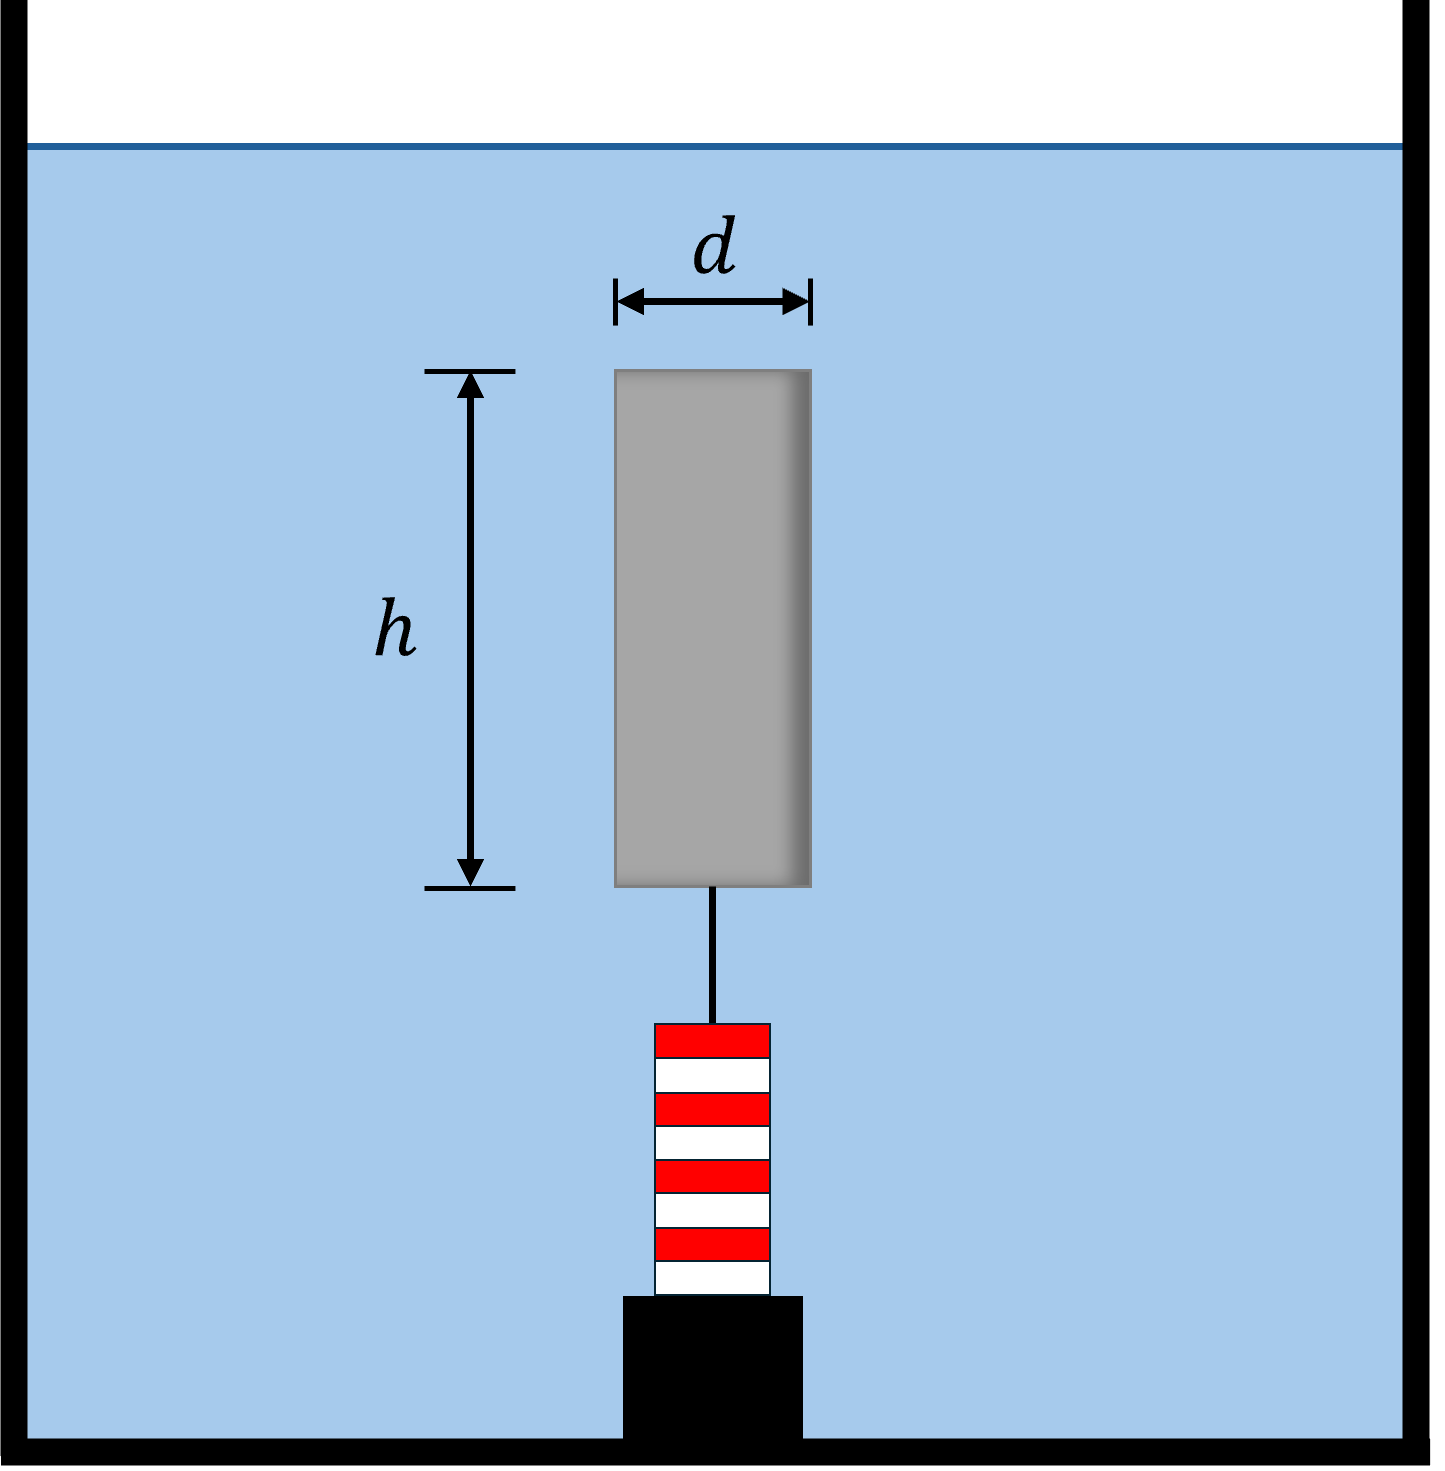
\includegraphics[width=0.4\textwidth]{Bilder/Test/SS2026/ZylinderUnterwasser.png}
\end{center}
Ein massiver Aluminiumzylinder mit Durchmesser $d = \SI{8.0}{\centi\metre}$ und Höhe $h = \SI{12.0}{\centi\metre}$ hängt an einem Federkraftmesser und ist vollständig in Wasser eingetaucht. Die Dichte von Aluminium beträgt $\rho_{\text{Al}} = \SI{2700}{\kilogram\per\metre\cubed}$, die Dichte von Wasser $\rho_{\text{W}} = \SI{1000}{\kilogram\per\metre\cubed}$ und die Erdbeschleunigung $g = \SI{9.81}{\metre\per\second\squared}$. Der Federkraftmesser sei für die Messung von Kräften unter Wasser kalibriert und kann sowohl positive als auch negative Werte anzeigen.

\subsection*{Aufgabe}
Berechnen Sie die Anzeige des Federkraftmessers, wenn der Zylinder in Ruhe vollständig unter Wasser hängt.

\subsection*{Vorgehen}
\begin{enumerate}
    \item Welche Kräfte wirken auf den Zylinder? Formulieren Sie die Bedingung für das Kräftegleichgewicht.
    \item Berechnen Sie das Volumen, die Masse und daraus die Gewichtskraft $F_G$ des Zylinders.
    \item Berechnen Sie die Auftriebskraft $F_A$ des Wassers auf den Zylinder.
    \item Stellen Sie die Gleichgewichtsbedingung auf und leiten Sie daraus eine Formel für die Federkraft $F_{\text{F}}$ her.
    \item Berechnen Sie die Anzeige des Federkraftmessers numerisch. Achten Sie dabei auf das Vorzeichen der Kräfte.
\end{enumerate}

\vfill
\begin{flushright}
\renewcommand{\arraystretch}{1.23}
\begin{tabular}{|c | c | c | c | c|}
\hline
\multicolumn{5}{|l|}{\textbf{\large{Punkte: \quad\quad\quad /13}}}\\
\hline
\textbf{1)} & \textbf{2)} & \textbf{3)} & \textbf{4)} & \textbf{5)} \\
\quad/1.5 & \quad/3 & \quad/2.5 & \quad/3 & \quad/3 \\
\hline
\end{tabular}
\end{flushright}

\newpage

\section*{Beispiel 4 - Single-Choice}
\textit{Beantworten Sie folgende Fragen. Sind Auswahlmöglichkeiten gegeben, ist nur eine Antwort pro Frage richtig.}

\begin{enumerate}[label=\arabic*.,itemsep=18pt]
    \item Welche physikalische Größe ist als Kraft pro Fläche definiert?
    \begin{itemize}[label={$\square$},itemsep=1pt,topsep=0pt]
        \item Energie
        \item Druck
        \item Arbeit
        \item Leistung
    \end{itemize}

    \item Welche Einheit hat die Dichte $\rho$ im SI-System?
    \begin{itemize}[label={$\square$},itemsep=1pt,topsep=0pt]
        \item \si{\kilogram\per\metre\cubed}
        \item \si{\newton\per\metre}
        \item \si{\joule\per\kilogram}
        \item \si{\pascal\second}
    \end{itemize}

    \item Welche Aussage ist bei einer gleichförmigen Kreisbewegung korrekt?
    \begin{itemize}[label={$\square$},itemsep=1pt,topsep=0pt]
        \item Die Richtung der Geschwindigkeit ist konstant.
        \item Die Zentripetalkraft ist gleich der Zentrifugalkraft.
        \item Der Betrag der Geschwindigkeit ist konstant.
        \item Die Beschleunigung ist null.
    \end{itemize}

    \item Welche Aussage zum Phasenübergang \gDQ{Schmelzen} ist richtig?
    \begin{itemize}[label={$\square$},itemsep=1pt,topsep=0pt]
        \item Beim Schmelzen sinkt die Temperatur zwangsläufig unter \SI{0}{\degreeCelsius}.
        \item Beim Schmelzen wird latente Wärme benötigt.
        \item Beim Schmelzen bleibt die innere Energie immer konstant.
        \item Beim Schmelzen wird keine Energie ausgetauscht.
    \end{itemize}

    \item Welche Formel beschreibt die Zentripetalkraft eines Körpers der Masse $m$, der sich mit der Geschwindigkeit $v$ auf einer Kreisbahn mit Radius $r$ bewegt?
    \begin{itemize}[label={$\square$},itemsep=1pt,topsep=0pt]
        \item $F = m g h$
        \item $F = m \frac{v^2}{r}$
        \item $F = pV$
        \item $F = \rho V g$
    \end{itemize}

    \item Welche Aussage zum 1. Newtonschen Axiom ist richtig?
    \begin{itemize}[label={$\square$},itemsep=1pt,topsep=0pt]
        \item Eine resultierende Kraft ist notwendig, damit ein Körper in Ruhe bleibt oder sich gleichförmig bewegt.
        \item Ohne resultierende Kraft bleibt ein Körper in Ruhe oder in gleichförmig geradliniger Bewegung.
        \item Kräfte treten immer paarweise auf.
        \item Wirkt eine Kraft, dann ist die Beschleunigung proportional zur Masse des Körpers.
    \end{itemize}

    \item In einer Flüssigkeit nimmt mit zunehmender Tiefe 
    \begin{itemize}[label={$\square$},itemsep=1pt,topsep=0pt]
        \item die Dichte zu.
        \item die Dichte ab.
        \item der Druck zu.
        \item der Druck ab.
    \end{itemize}

    \item Ein Körper verdrängt beim Eintauchen in Wasser ein Volumen von \SI{0.002}{\metre\cubed}. Wie groß ist die Auftriebskraft ungefähr bei $\rho_{\text{W}} = \SI{1000}{\kilogram\per\metre\cubed}$?
    \begin{itemize}[label={$\square$},itemsep=1pt,topsep=0pt]
        \item \SI{0.2}{\newton}
        \item \SI{2}{\newton}
        \item \SI{20}{\newton}
        \item \SI{200}{\newton}
    \end{itemize}

    \item Welche Einheit hat die Leistung?
    \begin{itemize}[label={$\square$},itemsep=1pt,topsep=0pt]
        \item \si{\joule}
        \item \si{\newton}
        \item \si{\watt}
        \item \si{\pascal}
    \end{itemize}

    \item Der Wirkungsgrad im Carnot-Kreisprozess hängt nur von der Temperatur des heißen und des kalten Reservoirs ab und lautet $\eta = 1 - T_{\text{kalt}}/T_{\text{heiß}}$. Wie maximieren Sie diesen Wirkungsgrad $\eta$ und was für technische Hürden ergeben sich dabei? 
    
\end{enumerate}

\vfill
\begin{flushright}
\renewcommand{\arraystretch}{1.23}
\begin{tabular}{|l c|}
\hline
\multicolumn{2}{|l|}{\textbf{\large{Punkte: \quad\quad\quad /10}}}\\
\hline
\textbf{1--10: je /1} & \\
\hline
\end{tabular}
\end{flushright}

\end{document}